\documentclass[aspectratio=169,xcolor=dvipsnames]{beamer}
\usetheme{SimplePlus}

\usepackage{babel}
\usepackage{hyperref}
\usepackage{graphicx}
\usepackage{float}
\usepackage{booktabs} % Allows the use of \toprule, \midrule and \bottomrule in tables

\title[short title]{Advanced Topics in Databases}
\subtitle{Data Warehouse / Warehousing (?)}

\author{Aníbal Silva \and Rui Fernandes}

\date{\today}

\setbeamertemplate{bibliography item}{\insertbiblabel}

%----------------------------------------------------------------------------------------
%	PRESENTATION SLIDES
%----------------------------------------------------------------------------------------

\begin{document}

\renewcommand{\today}{\ifcase \month\or January\or February\or March\or %
April\or May\or June\or July\or August\or September\or October\or November\or %
December\fi, \number \year}

\begin{frame}
    \titlepage
\end{frame}

\begin{frame}{Overview}
    \tableofcontents
\end{frame}

\section{Number of athletes by age}
\begin{frame}{Number of athletes by age}
    \begin{figure}[H]
        \centering
        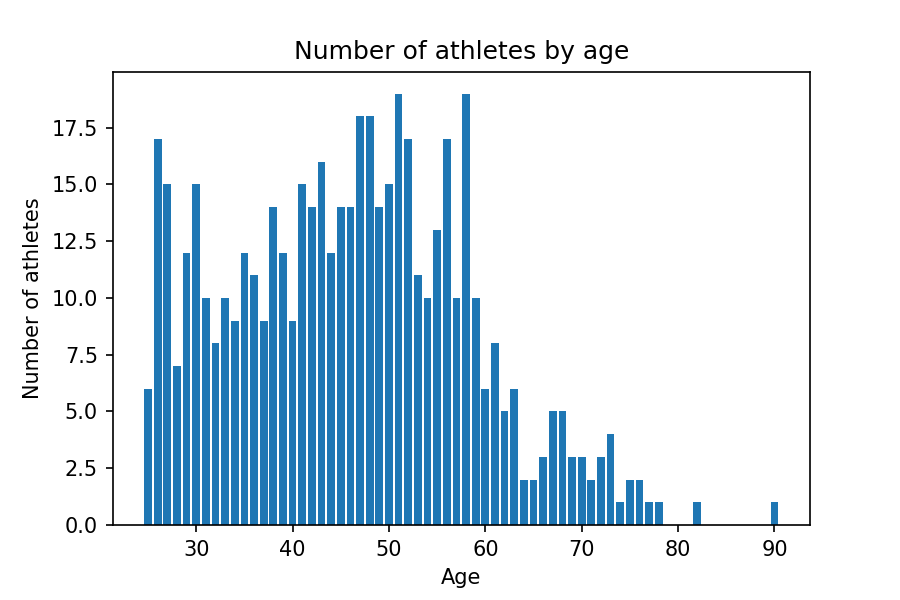
\includegraphics[width=.7\textwidth]{img/athletesbyage.png}
    \end{figure}
\end{frame}

\end{document}